\RequirePackage{xcolor}
\documentclass[journal,twoside,web]{ieeecolor}
\usepackage{jsen}
\usepackage{cite}
\usepackage{amsmath,amssymb,amsfonts}
\usepackage{graphicx}
\usepackage{textcomp}
\usepackage{wrapfig}
\usepackage{amssymb}
\usepackage{xcolor}
\usepackage{algorithmic}
\usepackage{array}
\usepackage{stfloats}
\usepackage{url}
\usepackage{epstopdf}
\usepackage{subfigure}
\usepackage{epsfig}
\usepackage{tikz}
\usepackage{dcolumn}
\usepackage{bm}
\usepackage{color}
\usepackage{accents}
\usepackage{braket}
\usepackage{mathtools}
\usepackage{tabularx}
\usepackage{nicefrac}
\usepackage{booktabs}
\usepackage{array}
\usepackage{multirow}
\usepackage[geometry]{ifsym}
\usepackage[T1]{fontenc}
\usepackage{cleveref}
%Definition of donde se dejan las imagenes
\graphicspath{ {./figures/} }
%Definition colour comments
\definecolor{javcolor}{rgb}{1.00, 0.0, 0.00}
\newcommand{\javnote}[1]{\textcolor{javcolor}{#1}}
%Definition colour
\definecolor{inicolor}{rgb}{0.0, 0.0, 1.00}
\newcommand{\ininote}[1]{\textcolor{inicolor}{#1}}
\definecolor{inacolor}{rgb}{0.0, 1.0, 1.00}
\newcommand{\inanote}[1]{\textcolor{inacolor}{#1}}
\newcommand*{\tikzbullet}[2]{%
  \setbox0=\hbox{\strut}%
  \begin{tikzpicture}
    \useasboundingbox (-.2em,0) rectangle (.2em,\ht0);
    \filldraw[draw=#1,fill=#2] (0,0.3\ht0) circle[radius=.2em];
  \end{tikzpicture}%
}
% Comando personalizado para cuadrados
\newcommand{\squarecolor}[1][black]{%
	\tikz\draw[fill=#1] (0,0) rectangle (0.2,0.2);%
}
\newcolumntype{N}{>{\centering\arraybackslash}m{.5in}}
\newcolumntype{M}{>{\centering\arraybackslash}m{0.7in}}
\newcolumntype{G}{>{\centering\arraybackslash}m{2in}}
\newcommand{\markerone}{\raisebox{0.5pt}{\tikz{\node[draw,scale=0.4,circle,fill=black!20!blue](){};}}}
\newcommand{\markertwo}{\raisebox{0pt}{\tikz{\node[draw,scale=0.3,regular polygon, regular polygon sides=3,fill=black!45!green,rotate=180](){};}}}
\newcommand{\markerthree}{\raisebox{0.5pt}{\tikz{\node[draw,scale=0.3,regular polygon, regular polygon sides=3,fill=black!10!red,rotate=0](){};}}}
\newcommand{\markerfour}{\raisebox{0.5pt}{\tikz{\node[draw,scale=0.4,regular polygon, regular polygon sides=4,fill=none](){};}}}
\newcommand{\markerfive}{\raisebox{0pt}{\tikz{\node[draw,scale=0.4,diamond,fill=black!10!gray](){};}}}
\newcommand{\markersix}{\raisebox{0.6pt}{\tikz{\node[draw,scale=0.3,circle,fill=black!100!](){};}}}
\def\BibTeX{{\rm B\kern-.05em{\sc i\kern-.025em b}\kern-.08em
    T\kern-.1667em\lower.7ex\hbox{E}\kern-.125emX}}
\markboth{\journalname, VOL. XX, NO. XX, XXXX 2022}
{Author \MakeLowercase{\textit{et al.}}: Preparation of Papers for IEEE TRANSACTIONS and JOURNALS (February 2017)}
\definecolor{abstractbg}{rgb}{0.89804,0.94510,0.83137}
\setlength{\fboxrule}{0pt}
\setlength{\fboxsep}{0pt}
\begin{document}
\title{Boosting the Performance of Planar CSRR Sensors in Biomedical Applications Through Machine Learning}
\author{Javier Alonso-Valdesueiro, Luis Fernández, Agustín Gutiérrez-Gálvez, and Santiago Marco-Colás
\thanks{J. Alonso-Valdesueiro is with University of Barcelona, Carrer Martí i Franquès,1. 08028, Barcelona, Spain (e-mail: javier.alonsov@ub.edu). }
\thanks{L. Fernández, is with University of Barcelona, Carrer Martí i Franquès,1. 08028, Barcelona, Spain (e-mail: lfernandez@ub.edu) and the Institute for Biomedical Engineering of Catalonia (IBEC), Carrer Baldiri i Reixac, 4, Torre R. 08028, Barcelona, Spain (email: lfernandez@ibecbarcelona.eu).}
\thanks{A. Gutiérrez-Gálvez, is with University of Barcelona, Carrer Martí i Franquès,1. 08028, Barcelona, Spain (e-mail: agutierrez@ub.edu).}
\thanks{S. Marco-Colás, is with University of Barcelona, Carrer Martí i Franquès,1. 08028, Barcelona, Spain (e-mail: santiago.marco@ub.edu) and the Institute for Biomedical Engineering of Catalonia (IBEC), Carrer Baldiri i Reixac, 4, Torre R. 08028, Barcelona, Spain (email: smarco@ibecbarcelona.eu).}}

\IEEEtitleabstractindextext{%
\fcolorbox{abstractbg}{abstractbg}{%
\begin{minipage}{\textwidth}%
\begin{wrapfigure}[18]{r}{3in}%
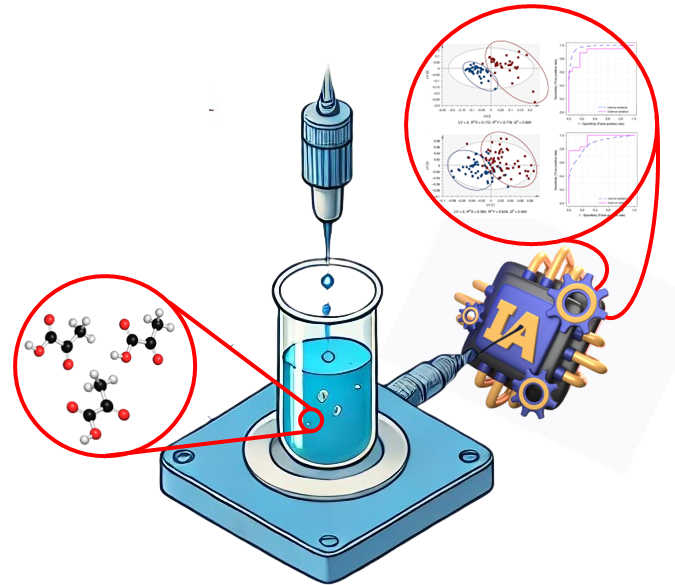
\includegraphics[width=2.5in]{figures/fig0.png}%
\end{wrapfigure}%
\begin{abstract}
Complementary Split Ring Resonators (CSRRs) have been widely explored as planar sensors over the last two decades. Despite their proven performance in laboratory settings — where high-end Vector Network Analyzers (VNAs) are employed, environmental conditions are monitored, and sampling methods are highly repeatible — their applicability outside controlled environments remains limited.

In this contribution, a novel approach is proposed to boost the practical applicability of CSRR sensors in biomedical research. The performance of a CSRR-based measurement system is measured by its capability of quantifying the concentration of a target substance in solution. Unlike conventional studies, the Scattering Parameters are measured using an inexpensive portable VNA, the SUT is placed inside standard test vials commonly used in biomedical laboratories, and no environmental control is applied during sampling. In this situation, it is demonstrated here that Machine Learning Algorithms enhances the performance of CSRR-based systems compared with traditional statistical analysis presented in the literature. 

Ethanol solutions diluted in clean water, ranging from $10\%$ to $96\%$ in concentration, were prepared and poured into commercial vials. A set of $90$ vials were prepared and measured by randomizing repetitions resulting in 500 samples in total — a sample size significantly larger than typically reported in the literature, aiming to enhance the robustness and reliability of the Machine Learning models.

Principal Component Analysis (PCA) was applied to the acquired dataset for exploring the underlying structure of the data. Subsequently, a Partial Least Squares Regressor (PLSR) was trained and validated using a Leave-One-Group-Out Cross-Validation scheme. The model achieved a Root Mean Square Error in Prediction (RMSEP) of approximately $3.7\%$ and a Limit of Agreement of approximately $15\%$ within a $95\%$ Confidence Interval — without exhibiting signs of underfitting or overfitting. These results highlight the potential of CSRR-based sensors for the quantification of bi-component liquid mixtures under realistic, uncontrolled conditions for biomedical applications.			   
\end{abstract} 

\begin{IEEEkeywords}
CSRR Sensors, Machine Learning, RF Biomedical, Resonators.
\end{IEEEkeywords}
\end{minipage}}}
\maketitle
\section{Introduction}
\label{sec:intro}
\IEEEPARstart{C}{omplementary} Split Ring Resonators (CSRR) were introduced as metasurfaces and metamaterials~\cite{falcone2004, Baena2005}. They were designed to act as microwave stopband and notch filters, transmission lines, and antennas~\cite{GGarcia2005, Bonache2006, Mandal2006, Gil2007, Velez2008, Zhang2009}. However, due to their sharp behavior as filters and the influence of surface surroundings on their Scattering Parameters (S-Parameters)~\cite{Grzegorczyk2005, Stevanovic2006, Bonache2006}, they started to be used as sensors a few years after their first appearance~\cite{Boybay2012}. Since then, several applications have focused on measuring the complex permittivity of different materials~\cite{Song2013, Lee2014, Lee2014_2, Ansari2015, Standaert2017, Su2019}.

In the last seven years, CSRR sensors have been increasingly used in biomedical applications to measure the dielectric properties of different solutions and concentrations of solutes in solvents~\cite{Velez2018, Omer2021, Zhang2019}. Some applications have attracted particular attention during this period (such as glucose concentration quantification in water~\cite{Omer2021, Martinic2025}), but most studies have focused on developing CSRR sensors for microfluidic devices applied to various fields~\cite{Patel2022, Jiang2023, Liu2024, Zhang2024}.

The use of statistical learning tools (or Machine Learning algorithms) to enhance the performance of CSRR-based devices has also been explored over the past five years~\cite{Prakash2022, Harrison2020, Kazemi2022, Abdolrazzaghi2023}. These algorithms have been employed as fitting tools to generalize the dependence of certain features of the CSRR S-parameters (such as frequency resonances, magnitude values, and phase distortion)  on the dielectric properties of the samples~\cite{Martinic2025}. Moreover, in recent years, their use has expanded to include Multivariate Analysis (MVA) for correlating solute concentrations in water~\cite{Trovarello2024}.

However, the full potential of ML algorithms applied to data from CSRR sensors has not yet been fully explored. These algorithms can generate quantification models inmune (up to certain point) to the variability (or noise) present in sensor readings~\cite{Mitchell1997, Wold1987, Wold2001, Nirmal2021}. ML models are capable of identifying common features in the data that allow correlation with specific characteristics of the sample under test (SUT)~\cite{Loutchanwot2022}. 

In this contribution, the proposed benchtop device is designed to be portable and low-cost, which introduces uncertainties due to the CSRR sensor, the Vector Network Analyzer (VNA) used to measure the S-parameters, and the sampling methodology. Enhancing the performance of this device is achieved by the appliying ML algorithms, specifically Principal Component Analysis (PCA) and Partial Least Squares Regression (PLSR). Therefore, a massive effort on building a comprehensive database was carried out. That allowed to use training schemes such as Leave-One-Group-Out Cross-Validation (LOGO-CV) to train the PLSR model which resulted in a quatification model that neither underfits nor overfits the training data. 

The text is organized as follows: In Section~\ref{sec:csrrbenchTop}, the measurement system is described, including the main characteristics of the CSRR sensor and the low-cost VNA used to measure the on of the S-Parameters (S$_{21}$), the sampling methodology and the ML workflow to train the quantification PLSR model which. Section~\ref{sec:csrrPerformance} presents the visualization of the extensive database generated for model training and the main results obtained with traditional modeling of CSRR sensor performance. This section also presents the data exploration through PCA and the the intermediate results of the PLSR training process. At the end the performance on the trained PLSR is reported. In Section~\ref{sec:csrrEval}, the performance of the CSRR system in quantifying the concentration of components in a binary solution is analyzed and discussed in comparisson with the traditional curve fitting models. Finally, Section~\ref{sec:conclusion} summarizes the capabilities of CSRR-based systems as benchtop devices working in biomedical applications.        

\section{CSRR benchtop System}\label{sec:csrrbenchTop}
\subsection{System Block Diagram}\label{ssec:sysBlockD}

\begin{figure}[!ht]
	\centering
	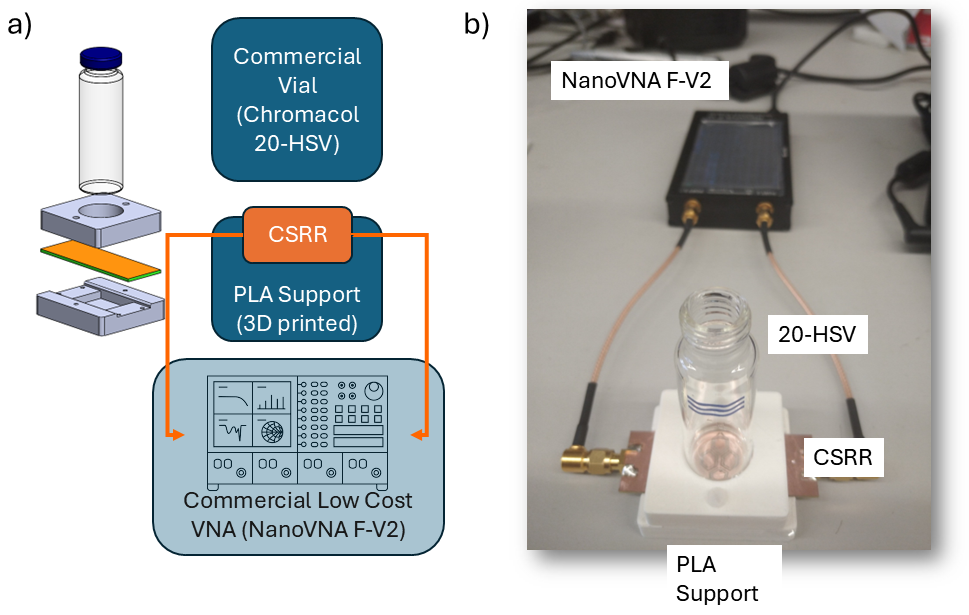
\includegraphics [trim = 0mm 0mm 0mm 0mm, clip, width=1\columnwidth]{figures/fig1.png}
	\caption{Proposed bench-top CSRR system. a) The commercial vial (Chromacol 20-HSV) containing the SUT is placed on the CSRR using a PLA 3D printed support. The CSRR is connected to the low cost VNA (NanoVNA F-V2) by two sma cables. The NanoVNA can be operated via graphical interface running in the device or serial commands coming from an application running in a common laptop. b) Real setup with a vial on top of the CSRR.}
	\label{fig:senBlockD}
	\vspace{-0.3cm}
\end{figure}

Figure~\ref{fig:senBlockD}~(a) shows the block diagram of the CSRR based system. The importance of describing the measurement system comes from the fact that, as it has been discussed in section~\ref{sec:intro}, in the literature, measurement systems are optimized for extracting the best performance of the sensors. 

In this contribution, the CSRR system is thought to be used as a bench-top tool in a biomedical laboratory. Therefore, the Sample Under Test (SUT) is presented to the sensor in a commercial vial (Chromacol 20-HSV). Its position on top of the sensor is ensured by a PLA holder 3D-printed. This holder keeps the CSRR still during measurements and ensures that the commercial vial is placed always centred with respect to the resonant structure of the CSRR sensor. 

The measurement device in a bench-top equipment, must be small, portable, and, if possible, affordable for being placed at any laboratory. In this case, the equipment must measure the S-parameters, in particular, the S$_{21}$. In some contributions, specific electronics were developed for the purpose of measuring this parameter~\cite{Omer2020, Omer2021}. In many other contributions, commercial, high quality and expensive devices are used~\cite{Patel2022, Jiang2023, Liu2024}. However, in this study, a commercial low-cost VNA was chosen as measurement platform (NanoVNA F-V2). This choice is based on the device  affordability, performance in the 1 to 3~GHz band, and operability with an external laptop via serial commands.

Finally, the VNA is connected to a controlling GUI developed in python and running in a commercial lap-top. The GUI allows to acquire data, record it in a comprehensive structure for generating a useful database and run in a continuous measurement mode. Also, it includes a quantification module to accommodate the resulting ML models after training and make predictions of concentration from measurements de S-parameter.   
\subsection{CSRR Sensor}
\label{ssec:csrrSensor}

\begin{figure}[!t]
	\centering
	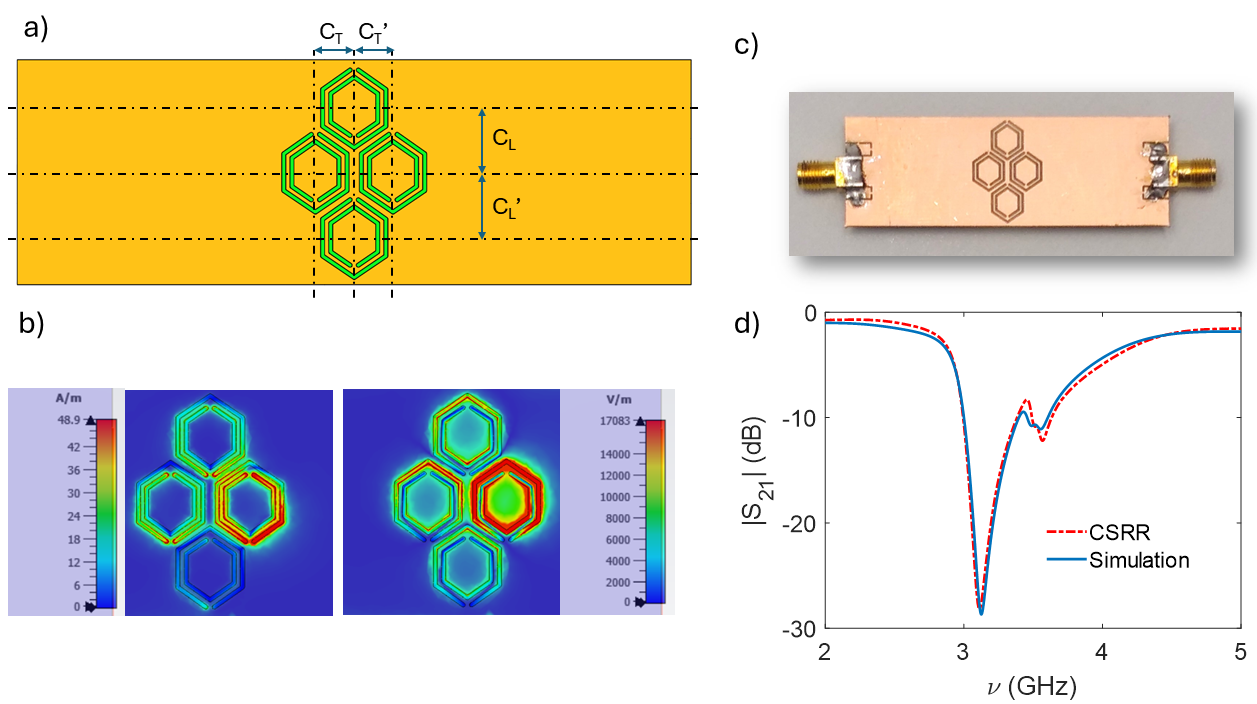
\includegraphics [trim = 0mm 0mm 0mm 0mm, clip, width=1\columnwidth]{figures/fig2.png}
	\caption{Modified CSRR. a) Structure of the measured CSRR with certain modifications. The honeycombs are not placed equidistantly to the centrer of the PCB ($22\times66$~mm). The longitudinal honeycombs are placed at C$_{L}=6.3$ and C$_{L}'=6.4$~mm away from the centrer of the PCB and the transverse honeycombs are placed C$_{T}=3.7$ and C$_{T}'=3.8$~mm away from the centrer of the PCB. b) Simulated electric ($\vec{E}$~\nicefrac{V}{m}) and magnetic field ($\vec{H}$~\nicefrac{A}{m}) in the surface of the multiple honeycomb structure. c) CSRR mounted with sma connectors. d) S$_{21}$ comparison between simulations and measurements when the CSRR is unloaded (Keisight E5071C-240).}
	\label{fig:csrr}
	\vspace{-0.3cm}
\end{figure}

Figure~\ref{fig:csrr}~(a) shows the structure of the CSRR used in this contribution and the PCB manufactured by Eurocircuits NV. Its structure is based on the honeycomb CSRR presented in~\cite{Omer2020}. However, in order to present some extra features in the S$_{21}$ parameter, some of its dimensions were modified. In particular, the symmetry of the vertical and horizontal combination of honeycombs was modified by 100~$\mu$m. This modification provided to CSRR with an extra feature ($\sim3.5$~GHz) close to the main resonance ($3.2$~GHz). This extra resonance comes from the fact that, the resonator presented here shows asymmetries in the horizontal and vertical plane. Therefore, it is expected to observe some directionality when measuring the S$_{21}$ with a SUT placed on top of the resonator.

The coupling transmission line and the dimensions of each honeycomb are as defined in~\cite{Omer2020}, so the CSRR does not introduce further uncertainty in the measurement.

\subsection{Sampling Methodology}
\label{ssec:samplingMethod}

\begin{figure*}[!t]
	\centering
	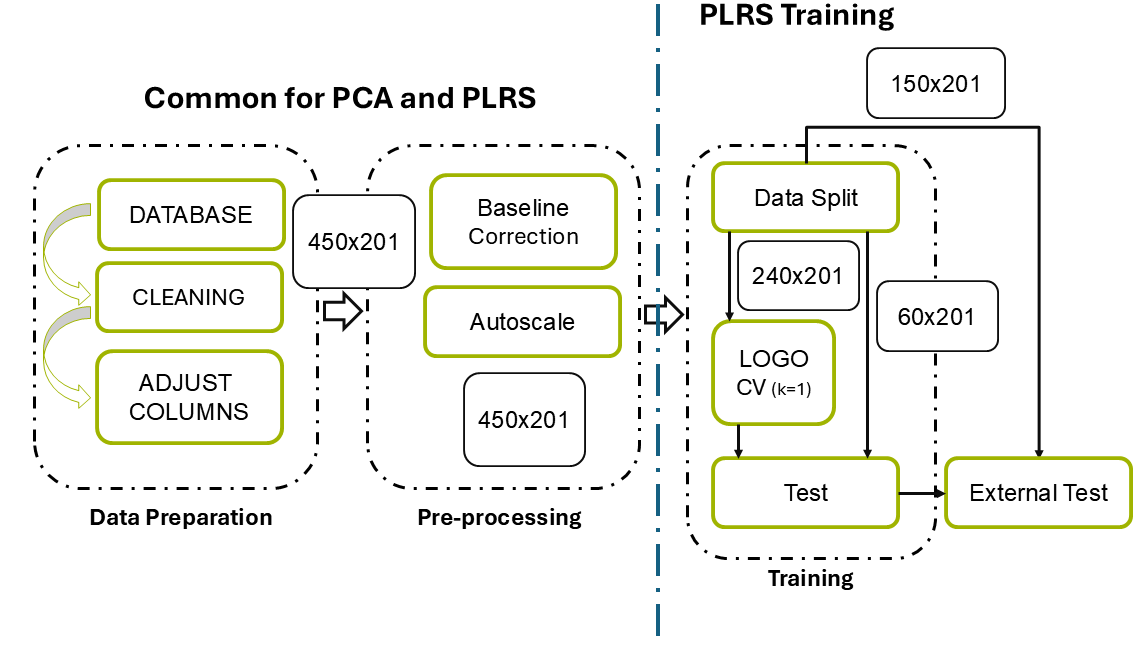
\includegraphics [trim = 0mm 0mm 0mm 0mm, clip, width=1.5\columnwidth]{figures/fig6_3.png}
	\caption{Block diagram of the developed workflow for training the bench-top CSRR system. In Data Preparation step, the database is cleaned by extracting the actual data (features) from metadata, providing a $450\times201$ feature matrix plus a $5\times201$ baseline matrix. In the Pre-Processing step the feature matrix baseline is correcte using the baseline matrix applied to each of the rounds separately. In the Training step, the feature matrix is split into the train dataset ($300\times201$ matrix) and the test dataset ($150\times201$ matrix). These two step are common for PCA and PLSR training algorithms. Then the train dataset is introduced in a leave-one-block-out cross-validation (LOGO-CV) training scheme which produces and optimized PLSR model. In the External Test step, the performance of the optimized model is evaluated by obtaining predictions from the test dataset.}
	\label{fig:workflow}
	\vspace{-0.3cm}
\end{figure*}

Sampling for training ML algorithms is a well established field in Statistical Learning. The main idea behind any sampling technique for ML model training is to randomize repetitions of each sample. This randomization mitigates undesired effects on the obtained dataset such as badge effects, repetition correlation and instrumental error propagation~\cite{Wu2020}. 

In this study, samples were organized by ethanol concentration in solution. The concentrations ranged from clean water (Ethanol at $0\%$) to Ethanol ($96\%$ purity) considering the steps depicted in figure~\ref{fig:avgData}~(a). Badge solutions were prepared with the mentioned concentrations and poured in $10$ commercial vials, chosen randomly from a pool of $100$ vials.

The $90$ vials were labelled for randomization and identification, and placed together for a day in a fridge at $5$~$^{\circ}$C. The day after, the vials were leaved out the fridge for an hour at $23$~$^{\circ}$C (temperature at the laboratory) and $5$ rounds of measurements were performed randomizing the order in which the vials were taken. Each round, consisted in ten repetitions of each concentration, where each repetition is a different vial. This provided a total of $100$ measurements. 
Before each round, the response of the CSRR sensor unloaded (S$_{21}$) was measured and used for baseline correction of the data. In total, $455$ measurements were taken for training and test of the ML model. Each measurement consisted in 201 points of recording the $20\dot{\log\left(|S_{21}|\right)}$ from $1.6$~GHz to $3$~GHz using the NanoVNA F-V2.
\subsection{Machine Learning Workflow}
\label{ssec:mlWorkflow}

 Pincipal Component Analysis (PCA) and Partial Least Squares Regressor (PLSR) are the two algorithms used for data analysis and model training in this contribution. The workflow is depicted in figure~\ref{fig:workflow} and described in the following sections.
\subsubsection{Principal Component Analysis}
\label{sssec:pca}

Principal Component Analysis (PCA) was performed on the 
database generated as explained in section~\ref{ssec:samplingMethod}. In this analysis, the dataset was prepared and pre-processed as depicted in figure~\ref{fig:workflow} and the PCA was performed using the Statistics and Machine Learning Toolbox from MATLAB. 

As it is shown in figure~\ref{fig:workflow}, the dataset is cleaned by extracting the metadata (labels, date of acquisition, etc.) of the database and adjusting the number of features of each repetition if necessary. Then, the data matrix ($450\times201$) is pre-processed in two steps. First, each round of measurements is corrected in its baseline by using the $20\dot{\log\left(|S_{21}|\right)}$ of the unloaded CSRR. Second, each $20\dot{\log\left(|S_{21}|\right)}$ is auto-scaled by calculating the average, $\mu_{C}$, and de standard deviation, $\sigma_{C}$, for each concentration at each round.

Up to $20$ PCs were considered for the analysis. The EV of the dataset was calculated for each PC and the cumulative EV was plotted. The distribution of the repetitions in the reduced vectorial space was also plotted for the first three PCs.  

\subsubsection{Partial Least Squares Regressor}
\label{sssec:pls}

The results from PCA analysis suggested that using every feature in the $20\dot{\log\left(|S_{21}|\right)}$ spectrum could lead to good results in quantification. The most extended predictor in this cases is the Partial Least Squares Regressor (PLSR), especially suitable for datasets with short number of repetitions per sample~\cite{Wold2001}.

Before starting the PLSR training, the feature matrix was pre-processed in the same way it was done for pca analysis (see figure~\ref{fig:workflow}). The pre-processed data is then split in two different subsets. The data belonging to $6$ concentrations is used for training (training dataset) and the rest is left aside for final testing (test dataset). Therefore, the training dataset consisted in a $300\times201$ feature matrix and the test dataset in a $150\times201$. 

A leave-one-block-out cross-validation (LOGO-CV) scheme is used for model training~\cite{Filzmoser2009}. This approach uses data from 4 rounds for model training and reserves one round for validation, resulting in 5 evaluations of different PLSR models. The model with best performance, in terms of Root Mean Square Error, is then selected. The LOGO-CV scheme is run for different number of Latent Variables up to 31. 

Once the PLSR model is trained, its evaluation is performed by introducing the test dataset and making predictions of the concentrations. In this case, predictions for $40\%$, $60\%$ and $80\%$ concentrations were calculated with the resulting model. These concentrations were chosen intentionally for compensating the presence of outliers (in $40\%$ for example) without having into account the both ends of the considered range.

\section{CSRR System Performance}
\label{sec:csrrPerformance}
In this section, the results from measurements, traditional characterization and ML analysis are presented. The performance of the CSRR system is evaluated in terms of the quantification of the concentration of ethanol in water. The results are discussed in terms of the traditional characterization of the system, the PCA analysis of the dataset and the performance of the PLSR model.

\subsection{Acquired Database}
\label{ssec:mlMeasurement}
\begin{figure}[!t]
	\centering
	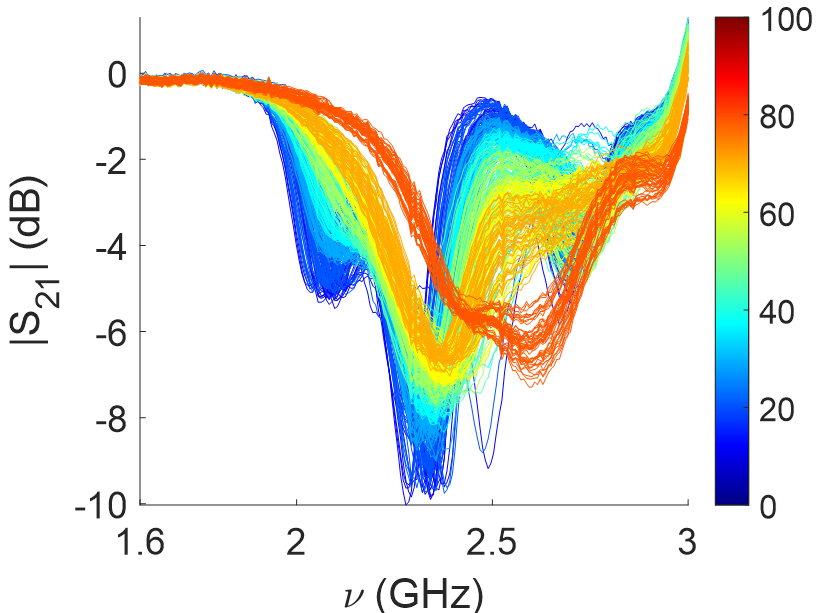
\includegraphics [trim = 0mm 0mm 0mm 0mm, clip, width=1\columnwidth]{figures/fig4_3.png}
	\caption{$20\dot{\log\left(|S_{21}|\right)}$ of each measurement contained in the generated dataset. Sampled concentrations of Ethanol in clean water ranges from $0\%$ and $96\%$. $10$ random commercial vials for each concentration were taken from a pool of $100$. $5$ rounds of measurements were performed. Each round consisted on measuring the $20\dot{\log\left(|S_{21}|\right)}$ of the CSRR when a random vial is picked and placed on top of the sensor, continuing and pass through the $90$ vials. Before each round, the $20\dot{\log\left(|S_{21}|\right)}$ of the CSRR unloaded was recorded for baseline correction of the data.}
	\label{fig:mlMeasTaken}
	\vspace{-0.3cm}
\end{figure}

Figure~\ref{fig:mlMeasTaken} shows the $20\dot{\log\left(|S_{21}|\right)}$ of each measurement contained in the dataset used for ML model training and test. Some features can be spotted by simple inspection. First, a wide dispersion of the curves is observed for each concentration. In particular, dispersion of deepest resonance seems to decrease with the concentration of ethanol. 

However, features around $2.1$~GHz and $2.5$~GHz show better discrimination between samples. Also, for $20\%$ of ethanol, two repetitions show an outlier behaviour with a $20\dot{\log\left(|S_{21}|\right)}$ out of the trend shown by rest of the dataset.  

Second, some outliers for certain concentrations ($0\%$, $20\%$ and $40\%$) were spotted in rounds $1$, $2$, $3$ and $5$. The repetitions corresponding to $40\%$ showed one outlier at each round, spotting a very different characteristics of the container vial with respect of the rest of the pool. However, the outliers from $0\%$ and $20\%$ where spotted at different rounds which points to different manipulation of the vials during measurement.

\subsection{Traditional System Characterization}
\label{ssec:sysCharac}
\begin{figure}[!t]
	\centering
	\subfigure{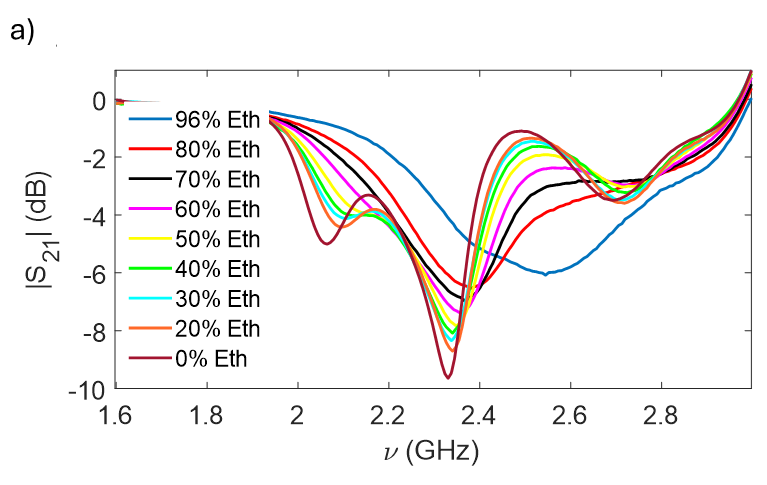
\includegraphics [trim = 0mm 0mm 0mm 0mm, clip, width=1\columnwidth]{figures/fig3_a.png}}
	\subfigure{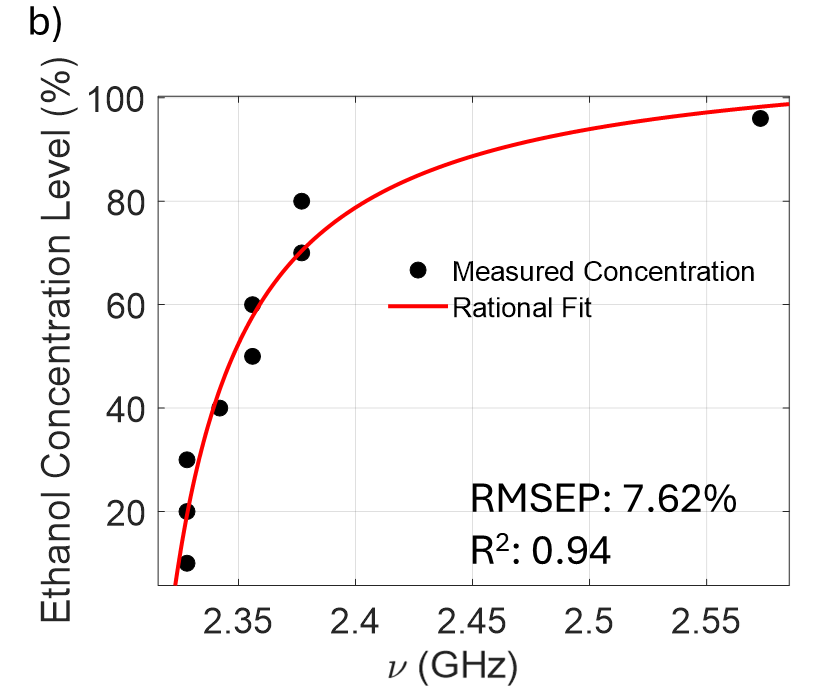
\includegraphics [trim = 0mm 0mm 0mm 0mm, clip, width=1\columnwidth]{figures/fig3_b.png}}
	%\hfill
	\caption{Traditional characterization of the CSRR system when measuring concentrations of ethanol diluted in clean water and poured in commercial vials. a) Averaged $20\dot{\log\left(|S_{21}|\right)}$ response of the generated database. b) Rational model for the frequency of the minimum observed in the averaged $20\dot{\log\left(|S_{21}|\right)}$ when every concentration of ethanol in clean water is observed ($10$, $20$, $30$, $40$, $50$, $60$, $70$, $80$, and $96$~$\%$)}
	\label{fig:avgData}
	\vspace{-0.3cm}
\end{figure}

Following the studies presented in the literature, figure~\ref{fig:avgData}~(a) shows the averaged $20\dot{\log\left(|S_{21}|\right)}$ for each concentration. It shows how the evolution of the shape of the S$_{21}$ parameter with the concentration implies a non-linear response of the system with ethanol. Evaluating the frequency displacement of the most prominent resonance in Figure~\ref{fig:avgData}~(a)~\cite{Abdolrazzaghi2023}, a rational fitting of the deepest resonance results in the following expression:

\begin{equation}
	\label{eq:frequFitt}
	 C_{\%}(\nu) = \frac{p1\cdot\nu+p2}{\nu+q} 
\end{equation} 

when the frequency,$\nu$ is in GHz and p1$=110.7274$~$\nicefrac{\%}{GHz^{2}}$, p2$=-257.0246$~$\nicefrac{\%}{GHz}$ and q$=-2.2893$~$GHz$. The R$^{2}$ of the fit is $0.9422$ and the RMSE$=7.9208$~$\%$. The fitting was performed using the Curve Fitting Toolbox from MATLAB. This model is presented in Figure~\ref{fig:avgData}~(b).

\subsection{Principal Component Analysis}
\label{ssec:pcaAnalysis}

\begin{figure}[!t]
	\centering
	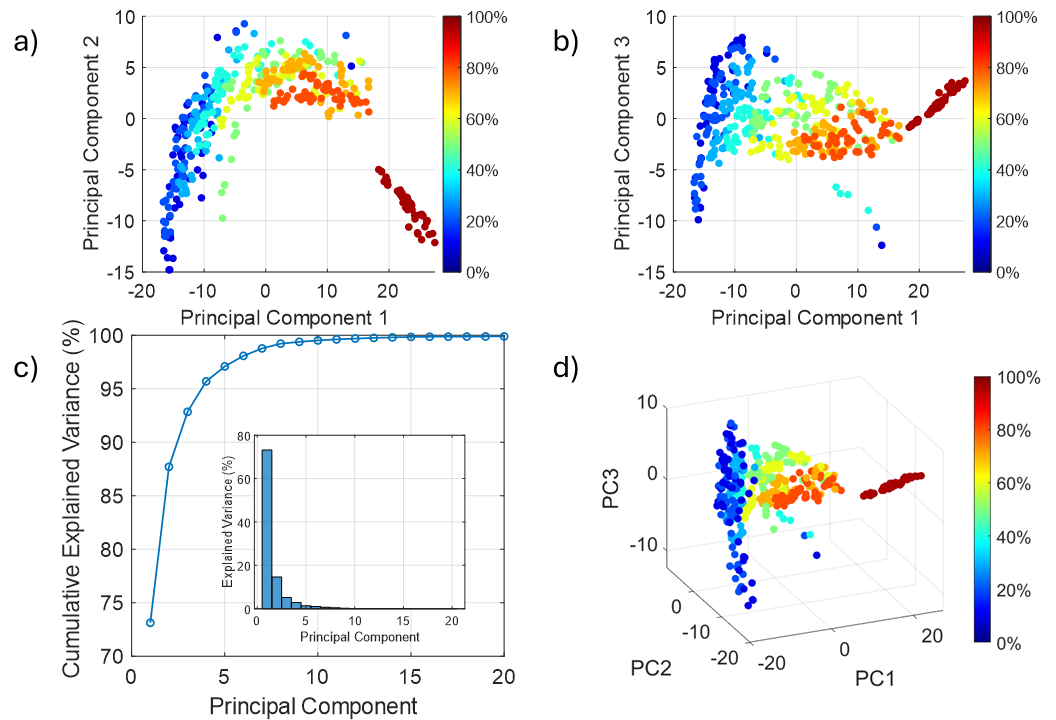
\includegraphics [trim = 0mm 0mm 0mm 0mm, clip, width=1\columnwidth]{figures/fig5_3.png}
	\caption{Principal Component Analysis (PCA) of the dataset generated as described in section~\ref{ssec:samplingMethod}. a) Distribution of each repetition in the reduced vectorial space when representing the second Principal Component (PC) with respect to the first PC. b) Distribution of each repetition in the reduced vectorial space when representing the third Principal Component (PC) with respect to the first PC. c) Cumulative Explained Variance of the dataset (in $\%$) with respect to the considered PCs and Explained Variance distribution over the set of PCs considered. d) 3D distribution of each repetition in the reduced vectorial space.}
	\label{fig:pcaAnalysis}
	\vspace{-0.3cm}
\end{figure}

Figures~\ref{fig:pcaAnalysis}~(a), (b) and (d), show the distribution of the repetitions in the reduced vectorial space of the extracted PCs. In both figures, the first PC shows its dominance which can be related with the ethanol concentration in solution. The spread in this component shows that, despite the careful preparation of each stock solution, the system is sensitive enough to observe relatively small variations in concentration. 

As shown by figure~\ref{fig:pcaAnalysis}~(c), the $95\%$ of the Explained Variance (EV) is contained in this first three Principal Components (PCs). Most of this variance is accumulated in the first PC ($73\%$), and the rest show an EV lower than $15\%$. 

Also, these figures show a spread in the second and third components which can be related to the variability introduced by the commercial vial and the actual measurement action (see figure~\ref{fig:pcaAnalysis}~(d)). Is in this variability where the outliers are observed. In particular, plot in figure~\ref{fig:pcaAnalysis}~(b) leads identify the outliers in concentrations of $0\%$, $20\%$ and $40\%$ shown in figure~\ref{fig:mlMeasTaken}.   


\subsection{Partial Least Squares Regressor Training}
\label{ssec:plsRegressor}

Once the workflow presented in figure~\ref{fig:workflow} is performed, there are certain intermediate results that provide ideas about the performance of the obtained model. Figure~\ref{fig:plsrStatistics}~(a) shows the evolution of the Root Mean Square Error (RMSE) with the number of components of the PLSR considered during the LOGO-CV scheme iteration. 

It is observed that with $6$ Latent Variables (LVs), the MSE of the best of the 5 models coming out from the LOGO-CV scheme is minimized up to $\sim6.8$ which leads to a Root Mean Square Error in Cross Validation (RMSECV) of $\sim3.62\%$.

Also, the most important features in the training dataset were observed by using the Variable Importance in Projection (VIP) scores per each of the features~\cite{Chong2005}. The calculated scores provide information of the averaged importance of each feature in the projection of the repetition in the restricted vectorial space that handles the PLSR. This information can be used to trim the feature matrix columns to the most relevant part of the $20\dot{\log\left(|S_{21}|\right)}$. There are many ways of defining the threshold that delimits which feature is more important than the rest~\cite{Ansari2015}. However, a good approach is to consider that every mean VIP score higher than $1$ belongs to a relevant feature. 
 
\begin{figure}[!t]
	\centering
	\subfigure{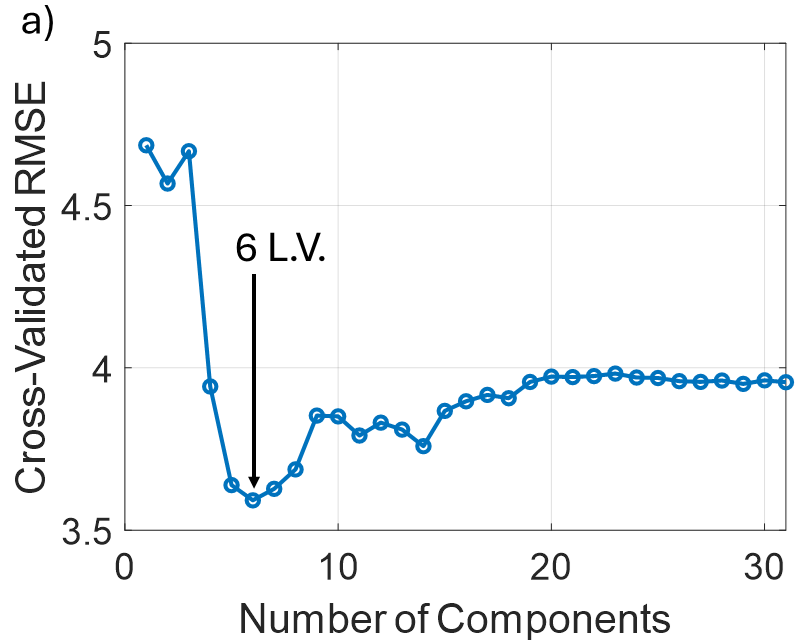
\includegraphics [trim = 0mm 0mm 0mm 0mm, clip, width=1\columnwidth]{figures/fig7_a.png}}
	\subfigure{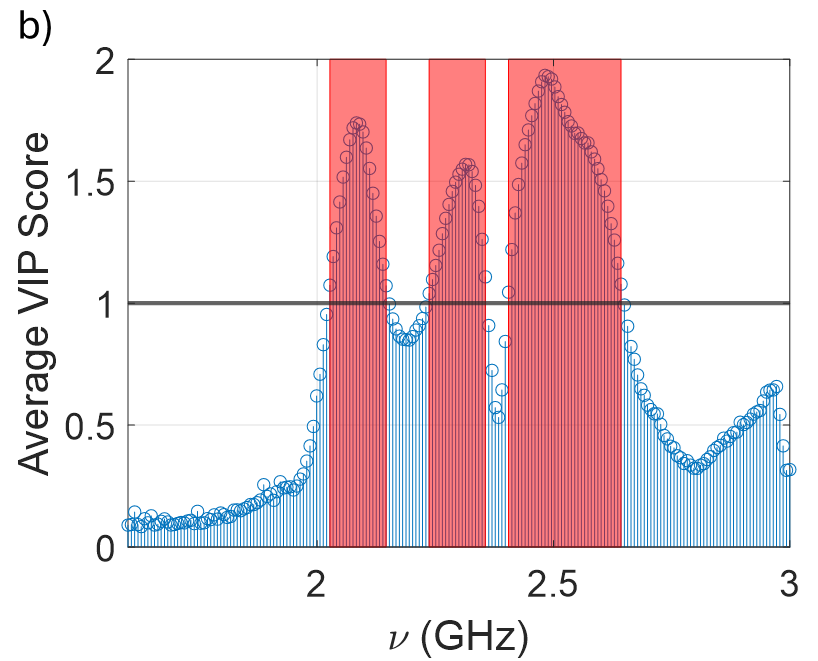
\includegraphics [trim = 0mm 0mm 0mm 0mm, clip, width=1\columnwidth]{figures/fig7_b.png}}
	%\hfill
	\caption{Statistics of the Partial Least Squares Regressor (PLSR) trained with the generated training dataset. a) Evolution of the Mean Square Error (MSE) with the number of Latent Variables (LV) during the Leave-One-Block-Out Cross Validation (LOGO-CV) training scheme. b) Mean Variable Importance in Projection (VIP) scores for each feature from $1.6$~GHz to $3$~GHz. The scores higher than $1$ have been highlighted with \squarecolor[pink].}
	\label{fig:plsrStatistics}
\end{figure}


Figure~\ref{fig:plsrStatistics}~(b) shows the VIP scores for the training dataset once the PLSR is optimized to $6$ LVs. In this figure, pink areas (\squarecolor[pink]) show scores $>1$. It is observed that most important parts of the $20\dot{\log\left(|S_{21}|\right)}$ correspond to data close to $2.1$~GHz, $2.45$~GHz and $2.5$~GHz. These frequency spans correspond to the most relevant differences between concentrations observed in figure~\ref{fig:mlMeasTaken}.

\subsubsection{Performance in Cross Validation}
\label{sssec:perfCV}

\begin{figure}[!t]
	\centering
	\subfigure{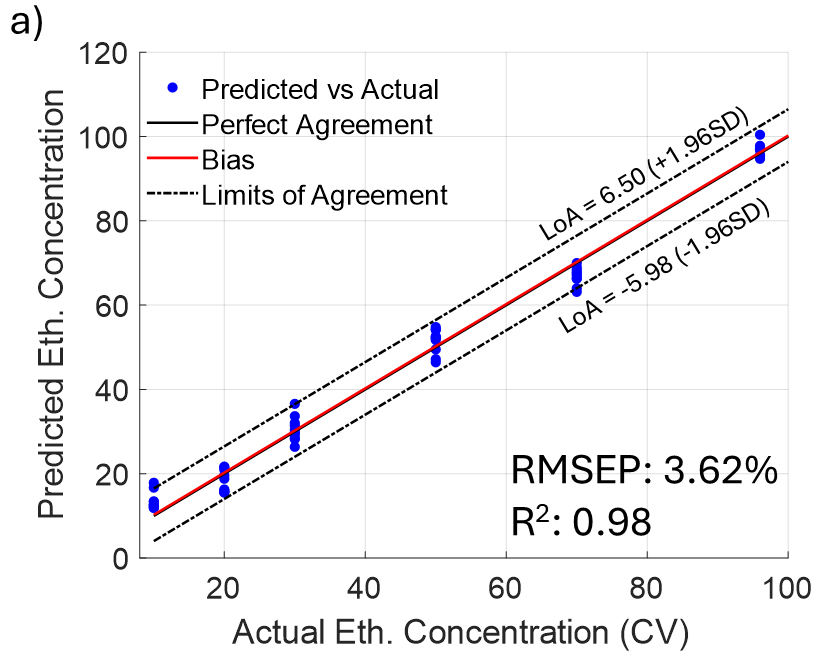
\includegraphics [trim = 0mm 0mm 0mm 0mm, clip, width=1\columnwidth]{figures/fig8_a.png}}
	\subfigure{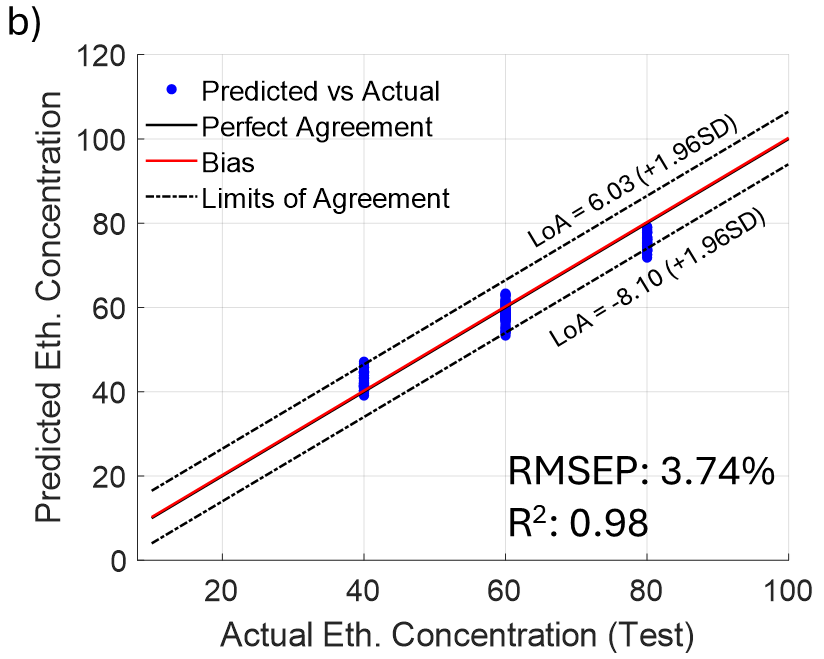
\includegraphics [trim = 0mm 0mm 0mm 0mm, clip, width=1\columnwidth]{figures/fig8_b.png}}
	%\hfill
	\caption{Statistics of the Partial Least Squares Regressor (PLSR) trained with the generated training dataset. a) Evolution of the Mean Square Error (MSE) with the number of Latent Variables (LV) during the Leave-One-Block-Out Cross Validation (LOGO-CV) training scheme. b) Mean Variable Importance in Projection (VIP) scores for each feature from $1.6$~GHz to $3$~GHz. The scores higher than 1 have been highlighted with \squarecolor[pink].}
	\label{fig:plsrResults}
\end{figure}

As mentioned in section~\ref{ssec:plsRegressor}, the LOGO-CV training scheme produces $5$ PLSR models per LVs considered during the training. From these $5$ models, the one with lower Root Mean Square Error (RMSE) is selected as representative of the LV set considered.

According with figure~\ref{fig:plsrStatistics}~(a), the PLSR model with $6$ LVs provides better performance during the LOGO-CV scheme. Therefore, this model was used to produce predictions on the training dataset. In this process, repetitions for $20\%$, $30\%$, $50\%$, $70\%$ and $96\%$ samples were part of the training dataset and the $20\%$ of these repetitions were kept aside for performance evaluation.

Figure~\ref{fig:plsrResults}~(a) shows the predictions of the PLSR model for the repetitions of the training dataset kept aside. The RMSE in CV (RMSECV) got close to $3.62$~$\%$ with R$^{2}$ coefficient of $0.98$. The Limits of Agreement (LoA) were calculated using Blant-Altmand method for the $95\%$ of Confident Interval resulting in $13.5\%$ deviation from linear prediction.
 
\subsubsection{Performance in Test}
\label{sssec:perfTest}

Despite the test during training is performed with repetitions that the LOGO-CV scheme had no access to, it is interesting to test if the PLSR model is able to predict concentrations that the training process have not seen before. 

In section~\ref{ssec:mlWorkflow}, the database was divided into training dataset and test dataset. The test dataset contained the repetitions of $40\%$, $60\%$ and $80\%$ samples. This dataset was used to obtain predictions with the PLSR model and evaluate its performance against "blind" samples.

Figure~\ref{fig:plsrResults}~(b) shows the predictions obtained for the test dataset. These predictions produced a RMSE in Prediction (RMSEP) about $3.7$~$\%$, very close to the RMSECV, with a R$^{2}$ coefficient of $0.98$. The LoAs were calculated in the same way presented in previous section, resulting in a LoA~$\sim14.2\%$ with a $95\%$ of Confident Interval. 

The PLSR models showed a $1.5\%$ bias when predicting the concentrations of the test dataset and the LoAs increased also $\sim1\%$ with respect to the LoAs obtained in training. 

These performance was a bit worse than the performance shown during training, but expected. The model was never put in contact with the data in the test dataset, therefore the variability of these samples (with their repetitions) might be different than the represented by the training dataset.

\section{CSRR System Evaluation}
\label{sec:csrrEval}

In this contribution, the impact of using Machine Learning Algorithms when measuring liquids with a CSRR based bench-top system is demonstrated. If properly applied, ML algorithms not only show the properties of the generated databases, but enhance the performance of low-cost bench top systems predicting concentrations of SUTs in samples.

For a bench-top system like the presented in section~\ref{sec:csrrbenchTop} the measurement procedure and the commercial vials used regularly in laboratories, introduce a considerable variability across repetitions. In the literature, this variability is managed, either enhancing the hardware of the system, which might be impossible in many of the cases due to the increase in hardware cost, or designing ad-hoc solutions specifically designed for reducing variability, as it happens with the vials used in the experiments~\cite{Omer2020, Omer2021}. 

However, it has been demonstrated in section~\ref{ssec:sysCharac} that repeating measurements of samples, even considering different vials, results in datasets with large standard deviations and it is expected that a simple curve fitting will fail in predicting the concentration of the SUT. In particular, the presented system, measurement procedure and commercial vials resulted in a curve-fitting based model with an RMSE of $7.62$~$\%$. These result shows that an univariant analysis of the S$_{21}$ parameter of the CSRR sensor is not enough for predicting the concentration of the SUT in these type of systems. If the system is used for biomedical applications in laboratories working as benchtop device a multivariate analysis is needed. 

As demonstrated in section~\ref{ssec:plsRegressor}, the application of ML algorithms might mitigate the observed lack of accuracy when using univariate models.  Furthermore, an oriented and extensive sampling ($455$ repetitions), that provides useful datasets (see section~\ref{ssec:mlMeasurement}), and a previous exploration of the obtained datasets, as explained in section~\ref{ssec:pcaAnalysis}, lead to a better understanding of the behaviour of CSRR bench-top systems. It also orientate to the proper prediction model useful for the application and the final use.

In particular, for the benchmark problem of ethanol concentration diluted in clean water, the PCA shows the variability of the dataset concentrated around 4 Principal Components (PCs), as it is shown in figure~\ref{fig:pcaAnalysis}. The first PC is clearly related to the ethanol concentration in the solution, while the rest of the PCs might be related to the variability introduced by the commercial vials and the measurement procedure. Furthermore, the training evolution of the PLSR model showed that 6 LVs minimized the RMSECV and the VIP scores analysis confirmed the multivariate nature of the problem.
 
In fact, the trained PLSR model trained with the workflow presented in section~\ref{ssec:mlWorkflow}, shows a better performance than the univariate model. In particular, a reduction by a factor of $\sim2$ in the RMSE at test (RMSEP $=3.74$~$\%$). Also, the LoAs are stable over the range of concentrations considered in the test dataset and very similar at training and test. This behaviour in training and test shows the robustness of the PLSR model compared with the quantification models presented in the literature. 

\section{Conclusions}
\label{sec:conclusion}
AS a result of the presented study, it has been demonstrated the enhancement of low-cost, benchtop, ready ot use in laboratories device performance by using Machine Learning algorithms, techniques and workflows. This demonstration was performed over a representative example using the benchmark problem of quantifying ethanol concentration diluted in clean water. The results show that and extensive sampling campaign and the use of ML algorithms, in particular PCA and PLSR, can improve the performance of traditional curve fitting by a factor of $2$.
These result overcome the limitations of the univariate analysis of the S$_{21}$ parameter of the CSRR-based system when working in real scenarios as biomedical laboratories. This opens the opportunity to use CSRR-based systems in biomedical applications as benchtop devices and move forward their development as usefull tools in screening, diagnosis or monitoring scenarios.

\section*{Acknowledgment}
Author want to thank Professor Antonio Pardo and Gema Guedes, Ph.D. for their collaboration during experiments in the laboratory and their understanding on the increasing entropy inside it.

\bibliographystyle{IEEEtran}
\bibliography{bib/ieeeBibCSRRandML}
%\vspace{-1cm}
\vskip -2\baselineskip plus -1fil

\begin{IEEEbiography}[{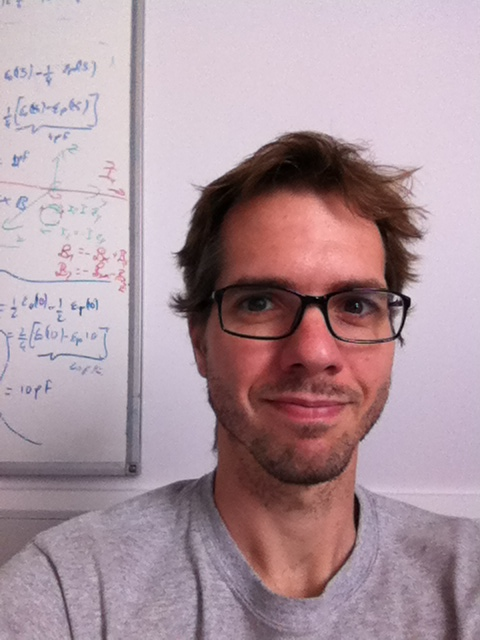
\includegraphics[width=1in,height=1.25in,clip,keepaspectratio]{figures/JAV-Website-Photo.jpg}}]{Javier Alonso-Valdesueiro}
was born in Madrid, Spain, in 1980. He earned a Telecommunications Engineering degree from the University of Alcalá, Madrid, in 2006, and a Ph.D. from the Polytechnic University of Catalonia, Barcelona, in 2011. From 2012 to 2020, he worked on developing electronic instrumentation for NMR experiments, initially at the C.E.A Center in France, followed by the University of Southampton in the UK, and later as a Marie Skłodowska-Curie Fellow at the University of the Basque Country (UPV/EHU). Over the past four years, he has advanced his career as an RF and instrumentation engineer in both private companies and public research centers, including TECNALIA Innovation Foundation and the Institute of Biomedical Engineering of Catalonia. Recently, he was appointed Assistant Professor in the Department of Electronic and Biomedical Engineering at the University of Barcelona. His current research focuses on radio-frequency (RF) devices for MRI, instrumentation electronics for gas sensing applications, and advancements in RF sensor technologies.
\end{IEEEbiography}
\vskip -2\baselineskip plus -1fil
%\vspace{-1.5cm}
\end{document}
